\section{Methods}
\label{c6:sec:methods}

\subsection{Study design and procedures}
The design of the Bio-SHiFT study has been described in detail elsewhere~\citep{van2018toward}. Briefly, CHF patients in clinically stable conditions were recruited during their regular outpatient visits in the Erasmus MC, Rotterdam, The Netherlands, and Northwest Clinics, Alkmaar, The Netherlands. Patients were eligible if CHF (with reduced or preserved ejection fraction) was diagnosed $\geq$~3 months ago according to the guidelines of the European Society of Cardiology~\citep{mcmurray2012v,paulus2007diagnose,dickstein2008stro}. Blood samples were taken on the day of inclusion and at predefined trimonthly follow-up visits, which were scheduled to a maximum follow-up duration of 30 months. Blood sampling and study procedures are further described in the Supplemental Materials. For the current investigation, we used 263 patients who were enrolled during the first inclusion period between October 2011 and June 2013. 

During follow-up, the occurrence of clinical events was recorded in the electronic case report forms, and associated hospital records and discharge letters were collected. Subsequently, a clinical event committee, blinded to the biomarker-candidate results, reviewed hospital records and discharge letters, and adjudicated the study endpoints. The primary study endpoint (PE) was defined as the composite of cardiac death, cardiac transplantation, left ventricular assist device implantation, or hospitalization for heart failure, whichever occurred first.

The Bio-SHiFT study was approved by the medical ethics committee of the Erasmus MC and was performed in accordance with the Declaration of Helsinki. Written informed consent was obtained from all patients. The Bio-SHiFT study is registered in ClinicalTrials.gov, number NCT01851538.

\subsection{Statistical analysis}
We utilized a joint model to estimate the association between longitudinally measured NT-proBNP and clinical outcome~\citep{rizopoulos2012joint,tsiatis2004joint}. A joint model combines a linear mixed-effect (LME) model for longitudinally measured data with a Cox regression model for time-to-event data. The association between these two types of data is modeled using patient-specific random effects. The LME model uses these random-effects to model the longitudinal temporal pattern of NT-proBNP measurements. The Cox model uses these random-effects to model the impact of the underlying trajectory of NT-proBNP measurements on the risk of PE~\citep{rizopoulos2016personalized,van2018toward}. The use of joint modeling is further motivated in Supplemental Materials. We used logarithmically (base 2) transformed NT-proBNP measurements in our joint model. Consequently, we were able to obtain a hazard ratio (HR) along with a 95\% confidence interval (CI) that estimated the risk of the PE associated with doubling of NT-proBNP level at a given follow-up time~\citep{van2018toward}.

The potential confounders that we used in our joint model were chosen based on their independent association with the PE in multivariable Cox regression models (NYHA class and diabetes mellitus) and existing literature (age, gender, renal function, body mass index). Covariates were missing in less than 3\% of the patients. Multiple imputations (5 times) of these covariates were performed in the multivariable analyses. 

\subsection{Scheduling personalized screening visits}
The scheduling of personalized screening visits is based on the individual patients' longitudinal biomarker profile. A patient visiting the outpatient clinic has longitudinal NT-proBNP measurements available until a certain time point. From the aforementioned joint model, we can derive for each individual patient the cumulative-risk of the PE at a particular follow-up time point, using all of the previously measured NT-proBNP up until this time point. 

For determining the optimal time point for drawing the next blood sample in a particular patient, we first need to establish the cumulative-risk of PE occurring in a certain time window. The time point for drawing the next blood sample should not be beyond the time point at which the PE occurs. For this reason, we set a maximum limit on the time window based on the cumulative-risk of the PE. Then, the time window is defined as the time between the current measurement and the maximum possible time point of drawing the next measurement. We aim to find the optimal time point to draw the next blood sample within this time window. We also need to define a risk threshold, which, if crossed within the time window, leads us to stop the further scheduling of measurements since the patient apparently needs appropriate action and/or increased surveillance, and therefore a different protocol from that point onwards. For this investigation, we have selected a risk threshold of 7.5\% for the three months that follow, based on clinical considerations. Thus, if the patients' cumulative-risk of the PE exceeds 7.5\% within the following three months, we stop scheduling further measurements in order to, for example, adjust therapy to avoid the occurrence of the PE. For the current investigation, we focus on the personalized screening schedules themselves, as our primary aim is to enable timely intervention before the occurrence of the PE. Hence, for now, we do not propose a specific therapy to be used at the time point that the patients' cumulative-risk of the PE exceeds the risk threshold. 

On the other hand, if the cumulative-risk of the PE remains less than 7.5\% within the following three months, we would like to determine the optimal time point at which to obtain the next NT-proBNP measurement. The selection of this optimal time point is based on two aspects.5 First, as stated, the cumulative-risk of PE in the time window should not exceed 7.5\%. Second, obtaining an NT-proBNP measurement at this optimal time point should provide us the maximum amount of information about the future cumulative-risk of PE for this particular patient. Accordingly, we perform personalized scheduling using the stepwise approach depicted in Figure~\ref{c6:fig:1}. Altogether, when applying this approach, patients with relatively stable biomarker profiles will likely not exceed the predefined risk threshold within a specified time window, and the calculations may suggest waiting for a longer time period to perform the next biomarker measurement in these patients. On the other hand, patients with worsening biomarker profiles are more likely to exceed the predefined risk threshold within a specified time window, and the calculations may suggest performing the next biomarker measurement in the short term.

\begin{figure}
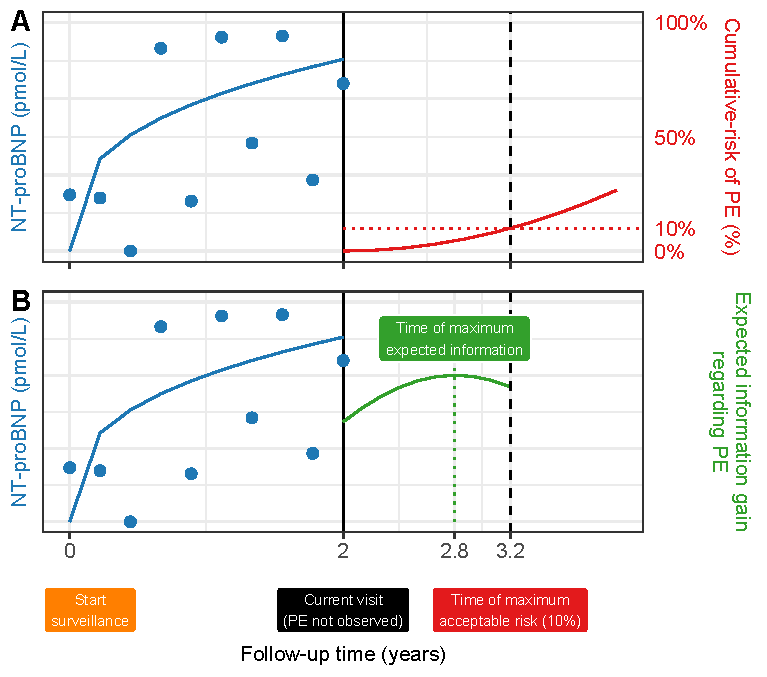
\includegraphics{contents/c6/images/c6_fig1.pdf}
\caption{\textbf{Illustration of personalized scheduling of biomarker measurements.} We plan NT-proBNP measurements until the cumulative-risk of PE (primary endpoint) at three months from the current visit is more than 10\%. \textbf{Panel~A}: Example patient with longitudinal NT-proBNP measurements and fitted profile (in blue). The time of the current visit, on which PE was not observed, is year 2. Using NT-proBNP and time of current visit data, we derive a personalized cumulative-risk profile for the patient (in red). This risk profile reaches the 10\% level at year 3.2, and hence, we are allowed to schedule new measurements until year 3.2. \textbf{Panel~B}: We calculate the expected information gain in the patient's prognosis if a new NT-proBNP measurement is done at a future time point between the current visit at year 2 and the time of the maximum acceptable risk of 10\% at year 3.2. The time of maximum expected information gain, is year 2.8, and hence, we schedule new NT-proBNP measurement at year 2.8.}
\label{c6:fig:1}
\end{figure}

\subsection{Simulation study}
After constructing the joint model and defining the thresholds needed for scheduling personalized screening visits, we proceeded to compare the personalized screening schedule to a fixed screening schedule. For the fixed schedule, we chose trimonthly intervals, in accordance with the design of the Bio-SHiFT study and daily clinical practice. Since our existing data were collected using this fixed screening schedule and hence no ‘real' data on personalized screening intervals was available, the advantages of a personalized screening design were assessed by means of a simulation study. 
We first simulated a dataset containing 750 patients. These 750 simulated patients had baseline characteristics and NT-proBNP profiles similar to the 263 patients included in the Bio-SHiFT since we simulated using the joint model fitted to the Bio-SHiFT data. We divided this data into training (700 patients), and testing (50 patients) set. For the training patients, using the joint model fitted to the Bio-SHiFT data, we generated NT-proBNP measurements at fixed follow-up time points. This schedule is similar to the schedule of the Bio-SHiFT study. We also generated a true PE time for these patients, as well as a random non-informative censoring time. Subsequently, we fitted a new joint model for these patients and, then, used this model to develop NT-proBNP measurement schedules for the test patients. To this end, in the test patients, we only generated the true PE time. Using such a design ensured that the ‘new' patients (n=50) are comparable to the ‘existing' patients (n=700) on which the model is based; if we had used the ‘real' patients (n=263 from the Bio-SHiFT study), this might not have been the case. 

Thus, for each of the 50 patients in the test set, we aimed to compare the efficacy of scheduling NT-proBNP measurements according to a fixed screening design and a personalized screening design. For the personalized screening design, the first three simulated NT-proBNP measurements were considered a given, in order to have a ‘run-in period' for the patients' longitudinal profile of NT-proBNP, since if we have a longitudinal profile available we can apply the aforementioned stepwise approach of personalized scheduling. Apart from using the risk-threshold of 7.5\% over a 3-month period, we repeated the analysis using 5\% and 10\% risk thresholds. We did so because 5\% is a lower cumulative-risk, and consequently, scheduling will stop earlier than in case of a 7.5\% risk threshold, which will give us more time to intervene with respect to the true PE time. Conversely, 10\% is a higher risk percentage than 7.5\%, and hence schedules based on the former will give us less time. 

The performance of the personalized and fixed screening schedules was compared using two outcome measures, namely, the start of the high-risk interval and the number of scheduled measurements. The high-risk interval was defined as the estimated intervention time minus the true event time (in months) (Fig. 1D). Thus, the schedule that showed a high-risk interval that was larger in absolute terms (i.e., more negative) was preferred, because such a high-risk interval enables timely intervention. In addition, assuming that the costs of NT-proBNP measurements and outpatient visits remained the same during follow-up, we prefer a procedure that requires the fewest possible repeated measurements (Supplemental Materials). All analyses were performed with R statistical software using package JMBayes~\citep{rizopoulosJMbayes}.